\section{導入と記号の定義}
\label{sec:introduction}
この章では adversarial examples がいかにして提案されたかという経緯と, 以降の章で必要となる記号やプログラム実行環境などの諸準備についてまとめる.



\subsection{導入}
\label{subsec:introduction}
adversarial examples は \cite{szegedy2013intriguing} によって初めて提案された.
これは人間には知覚しづらい摂動を入力データに加えて作成した新たな入力データのことを指し, 狭義\footnote{ここで狭義と言っているのは DNN 以外にも Support Vector Machine (SVM) や決定木や k Nearest Neighbor (kNN) に対する adversarial examples も考えられているためである \cite{papernot2016transferability}.この資料では DNN だけを対象にして, 他のモデルに対する adversarial examples は取り扱わない.}には Deep Neural Network (DNN) を誤認識させる性質を有するものである.
%
\begin{figure}[htbp]
\begin{center}
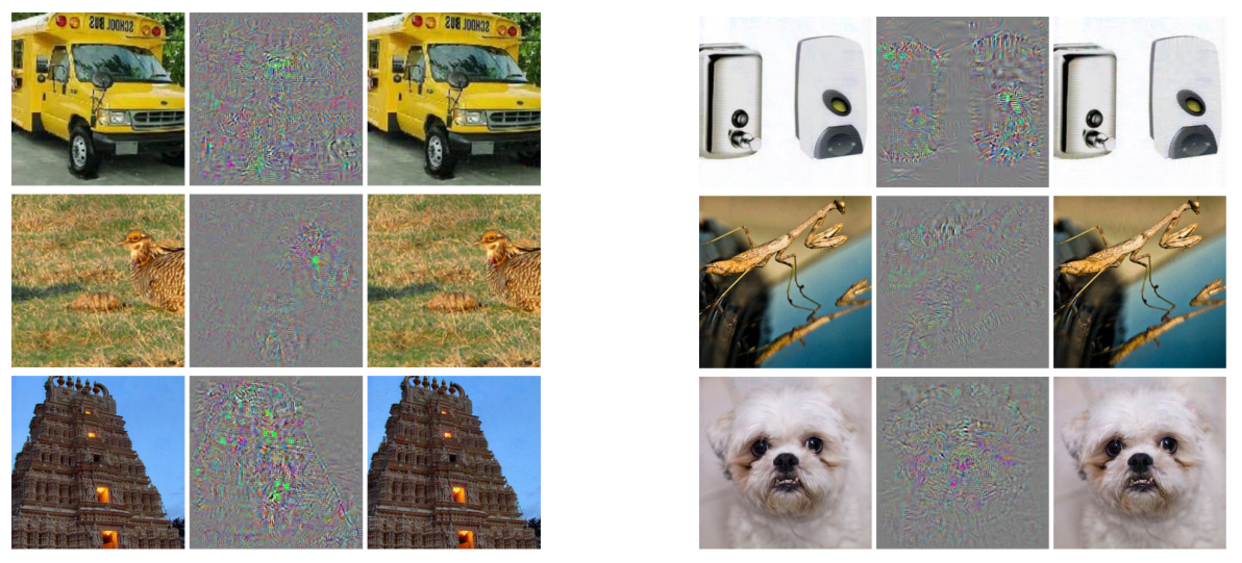
\includegraphics[width=12.0cm]{figures/szegedy-adv-examples.pdf}
\end{center}
\caption{adversarial examples の例.左列が元画像, 中央列が AlexNet \cite{krizhevsky2012imagenet} に対して生成された摂動, 右列が元画像に摂動を加えた画像である.
AlexNet は右列の画像に対して全て \textit{ostrich, Struthio camelus} (ダチョウ) と予測してしまう.図は \cite{szegedy2013intriguing} より引用.}
\label{fig:szegedy-adv-example}
\end{figure}
%

人間によるラベル予測や多くのカーネル法においては入力を少し変化\footnote{これは後に詳しく議論するが, あるノルムの意味で十分小さいと考えられる値で上から押さえられている摂動を入力に足すことを意味している.} させても出力には変化がなく (図 \ref{fig:szegedy-adv-example} の左列と右列は人間の目からは同じ対象物を表しているように見える), これを \cite{szegedy2013intriguing} では local generalization と呼んでる. このようなある種の「滑らかさ」は DNN においても成立するものと期待されていた.
しかし実際には図 \ref{fig:szegedy-adv-example} で示したように DNN においてはそのような期待が裏切られることが示された.
ある種の摂動が加えられた画像に対し, 人間の目には違いが見えづらいが, DNN は期待ところなる予測結果を返すという現象が発見されたのである.
その方法も誤認識させたいラベルに対する損失関数が小さくなるように準ニュートン法の Limited Broyden-Fletcher-Goldfarb-Shanno (L-BFGS) 法で摂動を見つけるというシンプルなものだったため, 多くの人々の興味を惹いた.

この論文の一年後に投稿された \cite{goodfellow2014explaining} ではよりシンプルな一階微分を用いた摂動を求める手法である Fast Gradient Sign Method (FGSM) が提案された.
これにより TensorFlow \cite{abadi2016tensorflow} を始めとする各種 DNN ライブラリでの扱いが容易になり, より多くの人にとって取り組みやすい対象となった.
研究が進むにつれて, adversarial examples は DNN の性質を探るという観点や実用上の脆弱性などの観点から大きく注目を集めるようになっていった.

DNN を用いたシステムやサービスを実際に運用するという立場から見ても, adversarial examples の存在は看過できないものである.
DNN はその予測性能の高さから様々なシステムに組み込まれるようになってきており, 顔認証や自動運転などはその代表例である.
自動運転のようにシステムのミスが人命に関わるような場合には品質保証は特に重要となるが, 映像から物体を認識するために DNN を使う場合は, adversarial examples による誤認識は実用に向けて大きな障壁となり得る.
同系統の議論として, DNN は予測の根拠が分かりづらいため説明可能性が必要だとする動きもあるが, adversarial examples は人間の期待と明白に異なる振る舞いを引き起こすものなので, より深刻であろう.

adversarial examples による攻撃は画像デジタルデータのピクセル値を直接変更する事に端を発したものであるが, その後の発展により物理的な環境下で対象物に摂動をプリントした紙やシールを貼る事で DNN を誤認識させることができるようになっているため, ここで述べている障壁は標語的なものではなく現実のものとなり得る.
悪意ある攻撃者が存在してもシステムを頑健に動作させるためにも, adversarial examples に関する理解を深めて適切に扱えるようになることは必要不可欠である.



\subsection{記号の定義}
\label{subsec:definition-symbols}
本書で使用する数学的な記号の定義を表 \ref{tb:notation} に列挙する.
入力データ $x$ に関しては height や width の次元を意識する必要性が生じる場面があまりないため, 必要なとき以外は単純に $\mathbb{R}^m$ の元として, 教師有りデータのラベルに関してはクラス数は $C$ とする.
本書では logit という言葉は softmax に入力する $C$ 次元のベクトルを指すものとする.
少し confusing な言葉遣いとして, logit というのは softmax に入力とするものを指す\footnote{
もともと logit 関数というのは sigmoid 関数の逆関数として定義されたものである: $\text{sigmoid} ( \text{logit}(p)) = p$.
これは任意の実数値を確率として解釈できる $[0, 1]$ に規格化するために sigmoid 関数がよく使われていたため, その逆関数に特別な名前を付与したことに由来する.
昨今では DNN が隆盛が甚だしく, DNN においては確率解釈のための規格化には softmax 関数が使われるため, logit という言葉が sotfmax 関数への入力を指すものとして使われることが増えてきた.
本書ではこの傾向に従い, softmax 関数への入力を logit と呼ぶことにする.
}.
モデルに関しては例えば $f_{\text{prob}} = \text{softmax} (f_{\text{logit}}(x))$ などの関係で結びつくものもあるが, 表記を簡潔にするため別個に定義している.
%
\begin{table}[htbp]
\begin{center}
\begin{tabular}{clccl}
\hline
表記  & 意味 & & 表記  & 意味 \\
\cline{1-2}
\cline{4-5}
$\mathcal{X}$ & 入力データ (画像) の集合 & & $x$ & $x \in \mathcal{X}$ なる要素で $x \in \mathbb{R}^m$ \\
& & & $x_{\text{adv}}$ & $x_{\text{adv}} = x + \omega$ なる adversarial example \\
$\mathcal{Y}$ & ラベルの集合 & & $y$ & $y \in \mathcal{Y}$ なる要素で $y \in \{1, 2, \dots, C\}$ \\
& & & $y_{\text{true}}$ & 入力データに対応する正しいラベル \\
& & & $y_{\text{atk-tgt}}$ & 摂動を加えることでモデルに誤認識させたいラベル \\
$\mathcal{D}_{\text{clean}}$ & 教師データの集合 & & $(x,y_{\text{true}})$ & 入力データとラベルの組からなる要素 \\
$\mathcal{D}_{\text{adv}}$ & adversarial データの集合 & & $(x_{\text{adv}},y)$ & 摂動を加えた入力データとラベルの組からなる要素 \\
$\Omega$ & 摂動の集合 & & $\omega$ & 入力データに加える摂動 ($x \rightarrow x + \omega$) で $\omega \in \mathbb{R}^m$ \\
& & & $\epsilon$ & 摂動の大きさをスカラー値で表現するもので $\epsilon \in \mathbb{R}_{+}$ \\
$\mathcal{F}$ & モデルの集合 & & & \\
& & & $f$ & 具体的な写像を考えずにモデルであることを示す \\
& & & $f_{\text{label}}$ & $f_{\text{label}}: x \rightarrow y$ なるモデル \\
& & & $f_{\text{prob}}$ & $x$ を入力として $C$ 次元のベクトルで確率を返す \\
& & & $f_{\text{logit}}$ & $x$ を入力として $C$ 次元のベクトルで logit を返す \\
& & & $f_{\text{bb}}$ & $x$ を入力として bounding box の情報を返す \\
$\mathcal{J}$ & loss function の集合 & & $J$ & $J: (f, x, y) \rightarrow v \in \mathbb{R}$ なる loss function  \\
& & & \\
& & & $\text{sign}$ & 符号関数 \\
& & & $\text{softmax}$ & softmax 関数: $p_i = \frac{\exp (f_{\text{logit}, i} (x))}{\sum_j \exp (f_{\text{logit}, j} (x))}$ \\
& & & $\text{softplus}$ & softplus 関数: $\ln (1 + \exp (x))$ \\
\hline
\end{tabular}
\caption{本書で使用する記号の定義. \label{tb:notation}}
\end{center}
\end{table}
%



\subsection{略語の定義}
\label{subsec:definition-abbreviations}
本書で使用する略語の定義を表 \ref{tb:abbreviation} に列挙する.
以降に出てくる略語は完全な表記を併記しないため, この表 \ref{tb:abbreviation} を参照すること.
例えば VGG は研究グループ名が特定のモデルを指す意味で使われるようになったもので, 略語だけ見ても何を指しているか分からないものも多いが, 慣例であるので致し方ない.
%
\begin{table}[htbp]
\begin{center}
\begin{tabular}{c|c}
\hline
略語 & 完全な表記 \\
\hline
bbox & bounding box \\
CIFAR & Canadian Institute For Advanced Research \\
CNN & Convolutional Neural Network \\
CW & Carlini-Wagner \\
DNN & Deep Neural Network \\
ELU & Exponential Linear Unit \\
Faster-RCNN & Faster-Regions with CNN features \\
FCN & Fully Convolutional Network \\
FGSM & Fast Gradient Sign Method \\
GAN & Generative Adversarial Network \\
ILSVRC & ImageNet Large Scale Visual Recognition Challenge \\
IoU & Intersection of Union \\
I+FGSM & Iterative Fast Gradient Sign Method \\
kNN & k Nearest Neighbor \\
L-BFGS & Limited Broyden-Fletcher-Goldfarb-Shanno \\
mAP & mean Average Precision \\
mIoU & mean IoU \\
MI+FGSM & Momentum Iterative Fast Gradient Sign Method \\
MLP & Multi-Layer Perceptron \\
MNIST & Modified National Institute of Standards and Technology \\
MSCOCO & Microsoft Common Objects in Context \\
NIN & Network In Network \\
NMS & Non Maximum Supression \\
R+FGSM & Randomized Fast Gradient Sign Method \\
PascalVOC & PASCAL Visual Object Classes \\
PGD & Projected Gradient Descent \\
RBF & Radial Basis Function \\
ReLU & Rectified Linear Unit \\
RPN & Region Proposal Network \\
SSIM & Structural SIMilarity \\
SVHN & Street View House Numbers \\
VGG & Visual Geometry Group \\
WGAN & Wasserstein GAN \\
ZF & Zeiler-Fergus\\
\hline
\end{tabular}
\caption{
本書で使用する略語の定義.
alphabetical に並べている.
\label{tb:abbreviation}
}
\end{center}
\end{table}
%



\subsection{検証プログラムに関する注意事項}
\label{subsec:note_on_code}
本書で使用するプログラムは GitHub レポジトリ \href{https://github.com/yoheikikuta/a-primer-on-adversarial-examples}{https://github.com/yoheikikuta/a-primer-on-adversarial-examples} で管理されている.
環境構築手順などは README.md に記載しているのでそちらを参照のこと.
基本的には docker \href{https://www.docker.com/}{https://www.docker.com/} を利用して Anaconda \href{https://www.anaconda.com/}{https://www.anaconda.com/} 環境を構築し, その上で PyTorch \cite{paszke2019pytorch} を使って実装をしている.
docker のインストール方法は公式ページ \href{https://docs.docker.com/install}{https://docs.docker.com/install} を参照のこと.
docker 環境が構築されていれば, git clone したレポジトリの top directory で下記コマンドを実行することで image の build と container の作成を実施できる.
%
\begin{lstlisting}[language=bash]
  $ docker build -t work -f Dockerfile .
  $ docker run --rm -it -v $PWD:/work work
  (do something in the container)
\end{lstlisting}
%

実行環境は基本的にローカルの PC で CPU を使用することを想定しているが, 計算負荷の大きい場面では \href{https://colab.research.google.com}{https://colab.research.google.com} の GPU 環境\footnote{
20200206 現在, Colaboratory では一回に最長 12 時間まで GPU/TPU を無料で使用できる.
notebook は放置していると仮想マシンから切断されて計算が止まってしまうため, 再接続を促されたらブラウザを操作して再接続をしたり, 定期的に notebook を開いているタブをリロードしたり, という必要がある.
この切断の時間間隔は以前は 90 分という話を聞くことが多かったが, 体感ではこの時間間隔は一定時間ではないようにも感じる (詳しく計測はしていない).
また, GPU は K80, T4, P4, P100 がランダムに割り当てられるとのことだが, 個人的には T4 か P100 のことが多い.
同じコードを実行しても割り当てられた GPU によって計算時間が変わってくるので注意が必要である.
詳しくは公式ページ \href{https://research.google.com/colaboratory/faq.html}{https://research.google.com/colaboratory/faq.html} を参照のこと.
有料だがより長時間使用したり良い GPU を優先的に使用できる Colab Pro も発表されているが, 20200206 時点では米国でのみ利用可能である.
}を使用している.
その際に使用した notebook ファイルも同梱している.